\documentclass[11pt, a4paper]{article}
\usepackage{pdfpages}
\usepackage{parallel}
\usepackage[T2A]{fontenc}
\usepackage{ucs}
\usepackage[utf8x]{inputenc}
\usepackage[polish,english,russian]{babel}
\usepackage{hyperref}
\usepackage{rotating}
\usepackage[inner=2cm,top=1.8cm,outer=2cm,bottom=2.3cm,nohead]{geometry}
\usepackage{listings}
\usepackage{graphicx}
\usepackage{wrapfig}
\usepackage{longtable}
\usepackage{indentfirst}
\usepackage{array}
\usepackage{tikzsymbols}
\usepackage{soul}
\usepackage[ruled,vlined]{algorithm2e}
%\counterwithout{figure}{section} 

\usepackage{url}
\makeatletter
\g@addto@macro{\UrlBreaks}{\UrlOrds}
\makeatother

\newcolumntype{P}[1]{>{\raggedright\arraybackslash}p{#1}}
\frenchspacing
\usepackage{fixltx2e} %text sub- and superscripts
\usepackage{icomma} % коскі ў матэматычным рэжыме
\PreloadUnicodePage{4}

\newcommand{\longpage}{\enlargethispage{\baselineskip}}
\newcommand{\shortpage}{\enlargethispage{-\baselineskip}}

\def\switchlang#1{\expandafter\csname switchlang#1\endcsname}
\def\switchlangbe{
\let\saverefname=\refname%
\def\refname{Літаратура}%
\def\figurename{Іл.}%
}
\def\switchlangen{
\let\saverefname=\refname%
\def\refname{References}%
\def\figurename{Fig.}%
}
\def\switchlangru{
\let\saverefname=\refname%
\let\savefigurename=\figurename%
\def\refname{Литература}%
\def\figurename{Рис.}%
}

\hyphenation{admi-ni-stra-tive}
\hyphenation{ex-pe-ri-ence}
\hyphenation{fle-xi-bi-li-ty}
\hyphenation{Py-thon}
\hyphenation{ma-the-ma-ti-cal}
\hyphenation{re-ported}
\hyphenation{imp-le-menta-tions}
\hyphenation{pro-vides}
\hyphenation{en-gi-neering}
\hyphenation{com-pa-ti-bi-li-ty}
\hyphenation{im-pos-sible}
\hyphenation{desk-top}
\hyphenation{elec-tro-nic}
\hyphenation{com-pa-ny}
\hyphenation{de-ve-lop-ment}
\hyphenation{de-ve-loping}
\hyphenation{de-ve-lop}
\hyphenation{da-ta-ba-se}
\hyphenation{plat-forms}
\hyphenation{or-ga-ni-za-tion}
\hyphenation{pro-gramming}
\hyphenation{in-stru-ments}
\hyphenation{Li-nux}
\hyphenation{sour-ce}
\hyphenation{en-vi-ron-ment}
\hyphenation{Te-le-pathy}
\hyphenation{Li-nux-ov-ka}
\hyphenation{Open-BSD}
\hyphenation{Free-BSD}
\hyphenation{men-ti-on-ed}
\hyphenation{app-li-ca-tion}

\def\progref!#1!{\texttt{#1}}
\renewcommand{\arraystretch}{2} %Іначай формулы ў матрыцы зліпаюцца з лініямі
\usepackage{array}

\def\interview #1 (#2), #3, #4, #5\par{

\section[#1, #3, #4]{#1 -- #3, #4}
\def\qname{LVEE}
\def\aname{#1}
\def\q ##1\par{{\noindent \bf \qname: ##1 }\par}
\def\a{{\noindent \bf \aname: } \def\qname{L}\def\aname{#2}}
}

\def\interview* #1 (#2), #3, #4, #5\par{

\section*{#1\\{\small\rm #3, #4. #5}}
\ifx\ParallelWhichBox\undefined%
    \addcontentsline{toc}{section}{#1, #3, #4}%
\else%
\ifnum\ParallelWhichBox=0%
    \addcontentsline{toc}{section}{#1, #3, #4}%
\fi\fi%

\def\qname{LVEE}
\def\aname{#1}
\def\q ##1\par{{\noindent \bf \qname: ##1 }\par}
\def\a{{\noindent \bf \aname: } \def\qname{L}\def\aname{#2}}
}

\newcommand{\interviewfooter}[1]{
\vskip 1em
\noindent \textit{#1}
}

\switchlang{en}
\begin{document}

\title{1993 "--- Easy Options trackball}
\date{}
\maketitle
\selectlanguage{english}
The most notable visual feature of the Easy Options trackball is the 60s home appliance style design (figure \ref{fig:EasyOptionsPic}).

\begin{figure}[h]
    \centering
    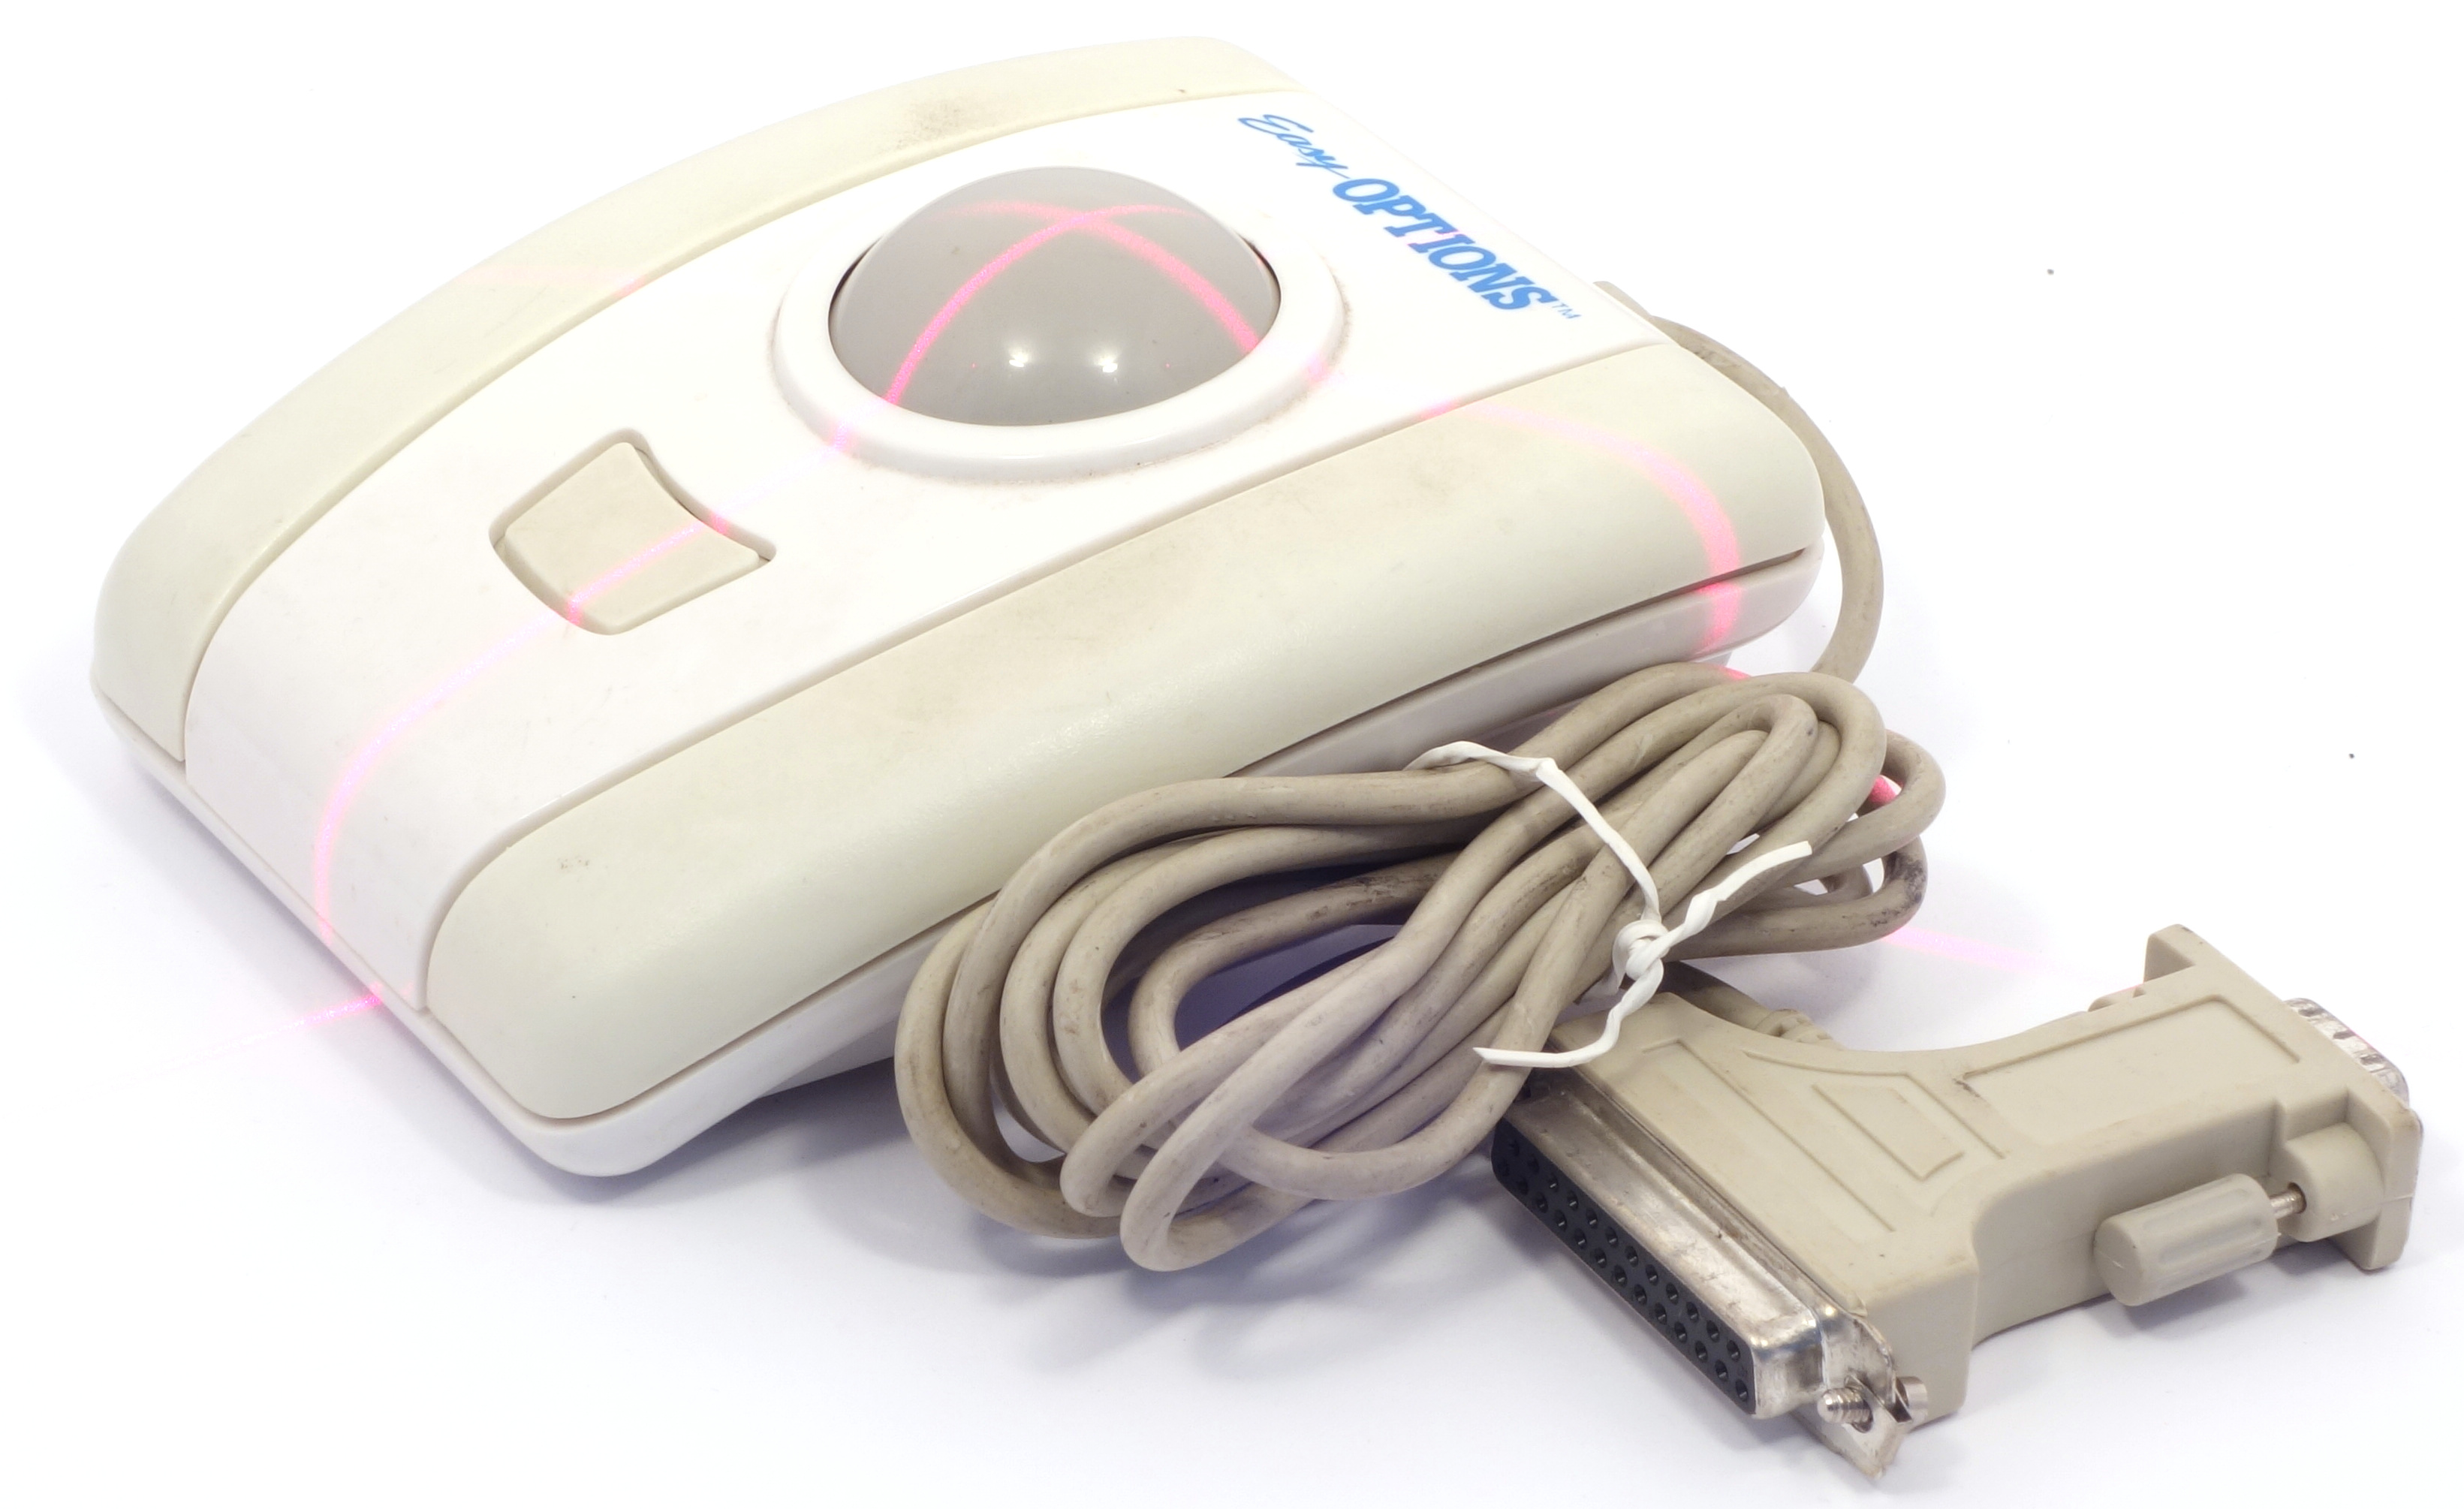
\includegraphics[scale=0.7]{1993_easy_options_trackball/pic_60.jpg}
    \caption{Easy Options trackball}
    \label{fig:EasyOptionsPic}
\end{figure}

Turning the device upside down shows the FCC ID code (figure \ref{fig:EasyOptionsTopBottom}), which reveals that the trackball has been manufactured by a Taiwanese company since 1993.

\begin{figure}[h]
    \centering
    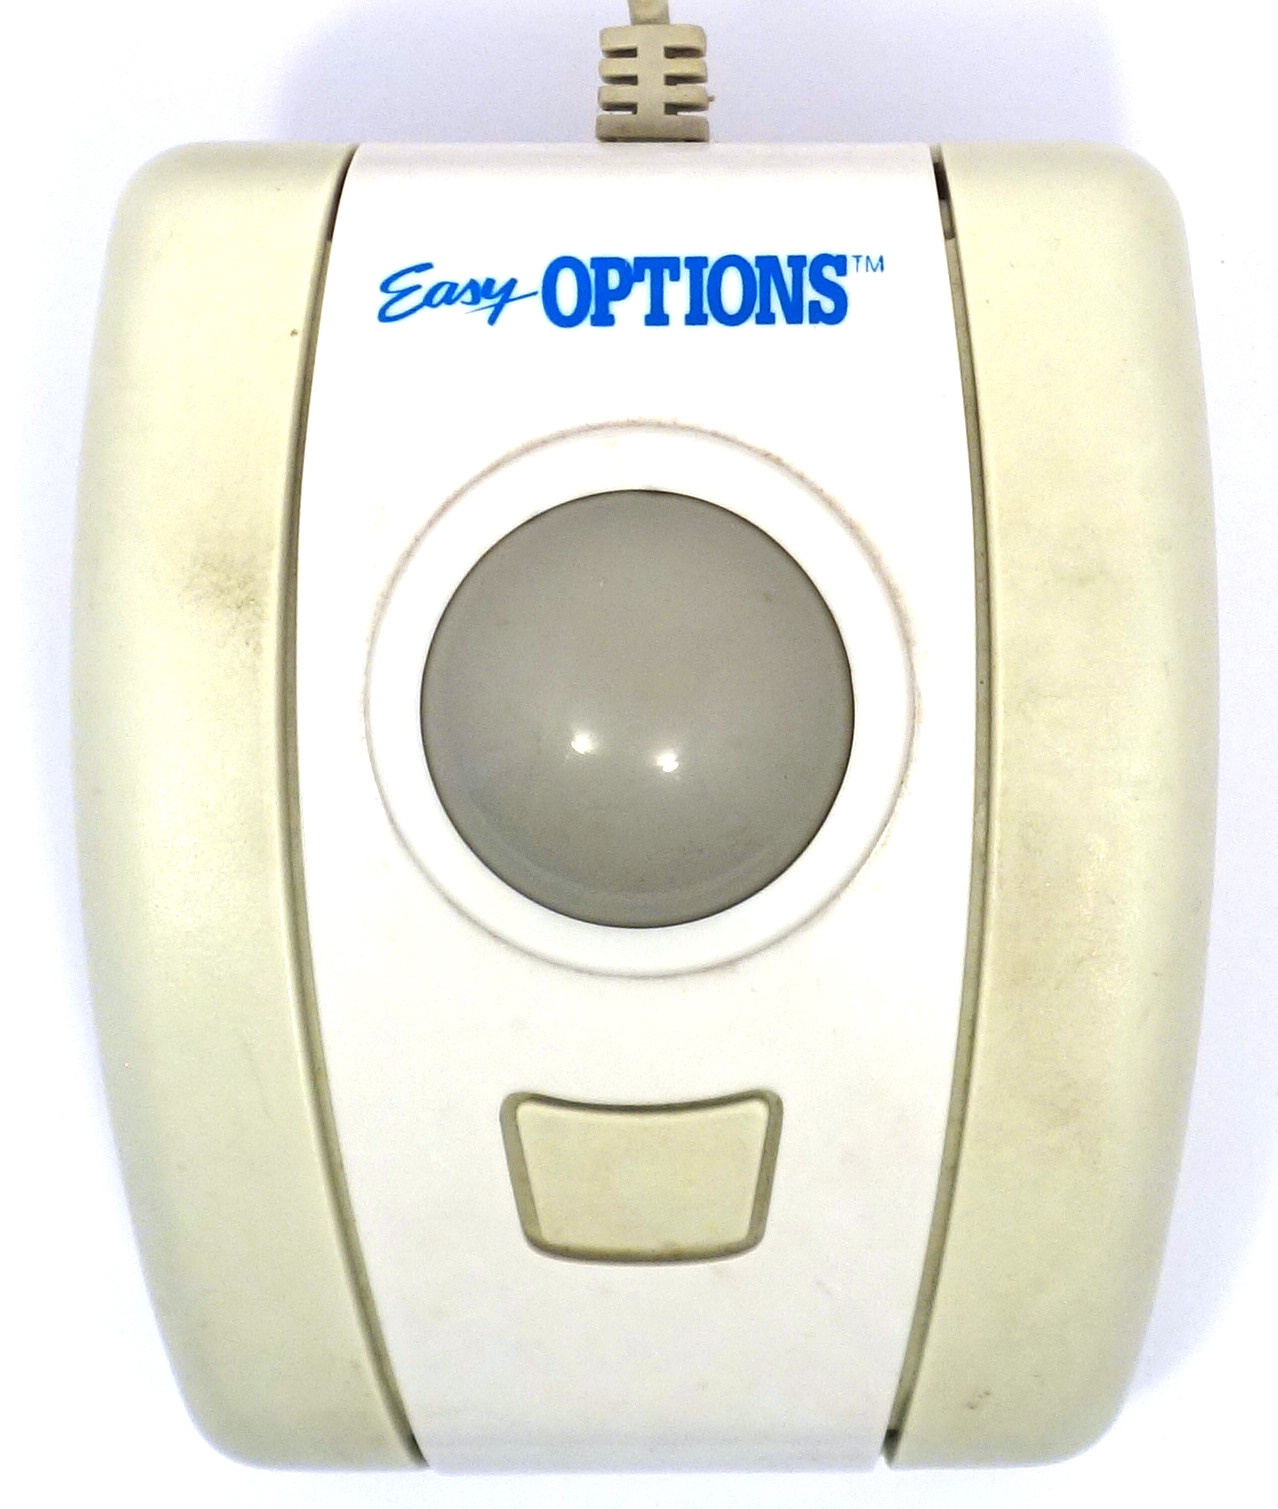
\includegraphics[scale=0.6]{1993_easy_options_trackball/top_60.jpg}
    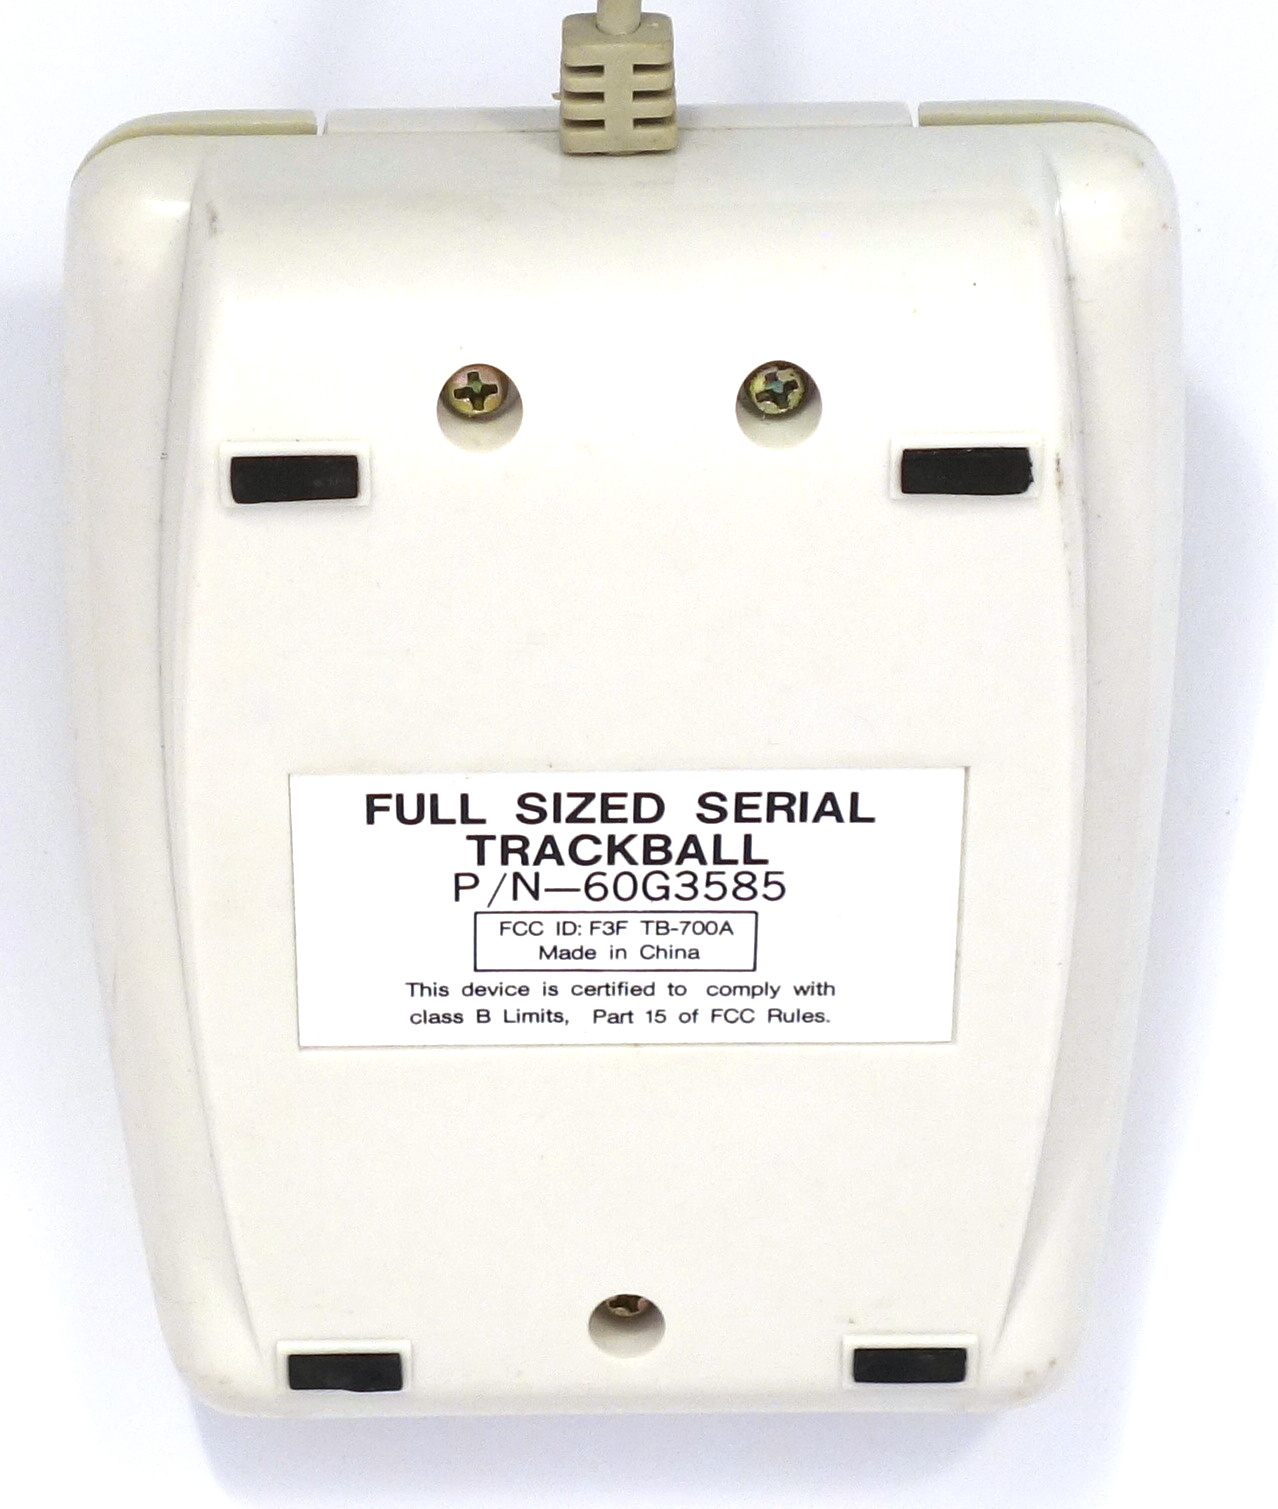
\includegraphics[scale=0.6]{1993_easy_options_trackball/bottom_60.jpg}
    \caption{Easy Options, top and bottom views}
    \label{fig:EasyOptionsTopBottom}
\end{figure}

As you can see in figure \ref{fig:EasyOptionsSize}, this manipulator is relatively small.

\begin{figure}[h]
    \centering
    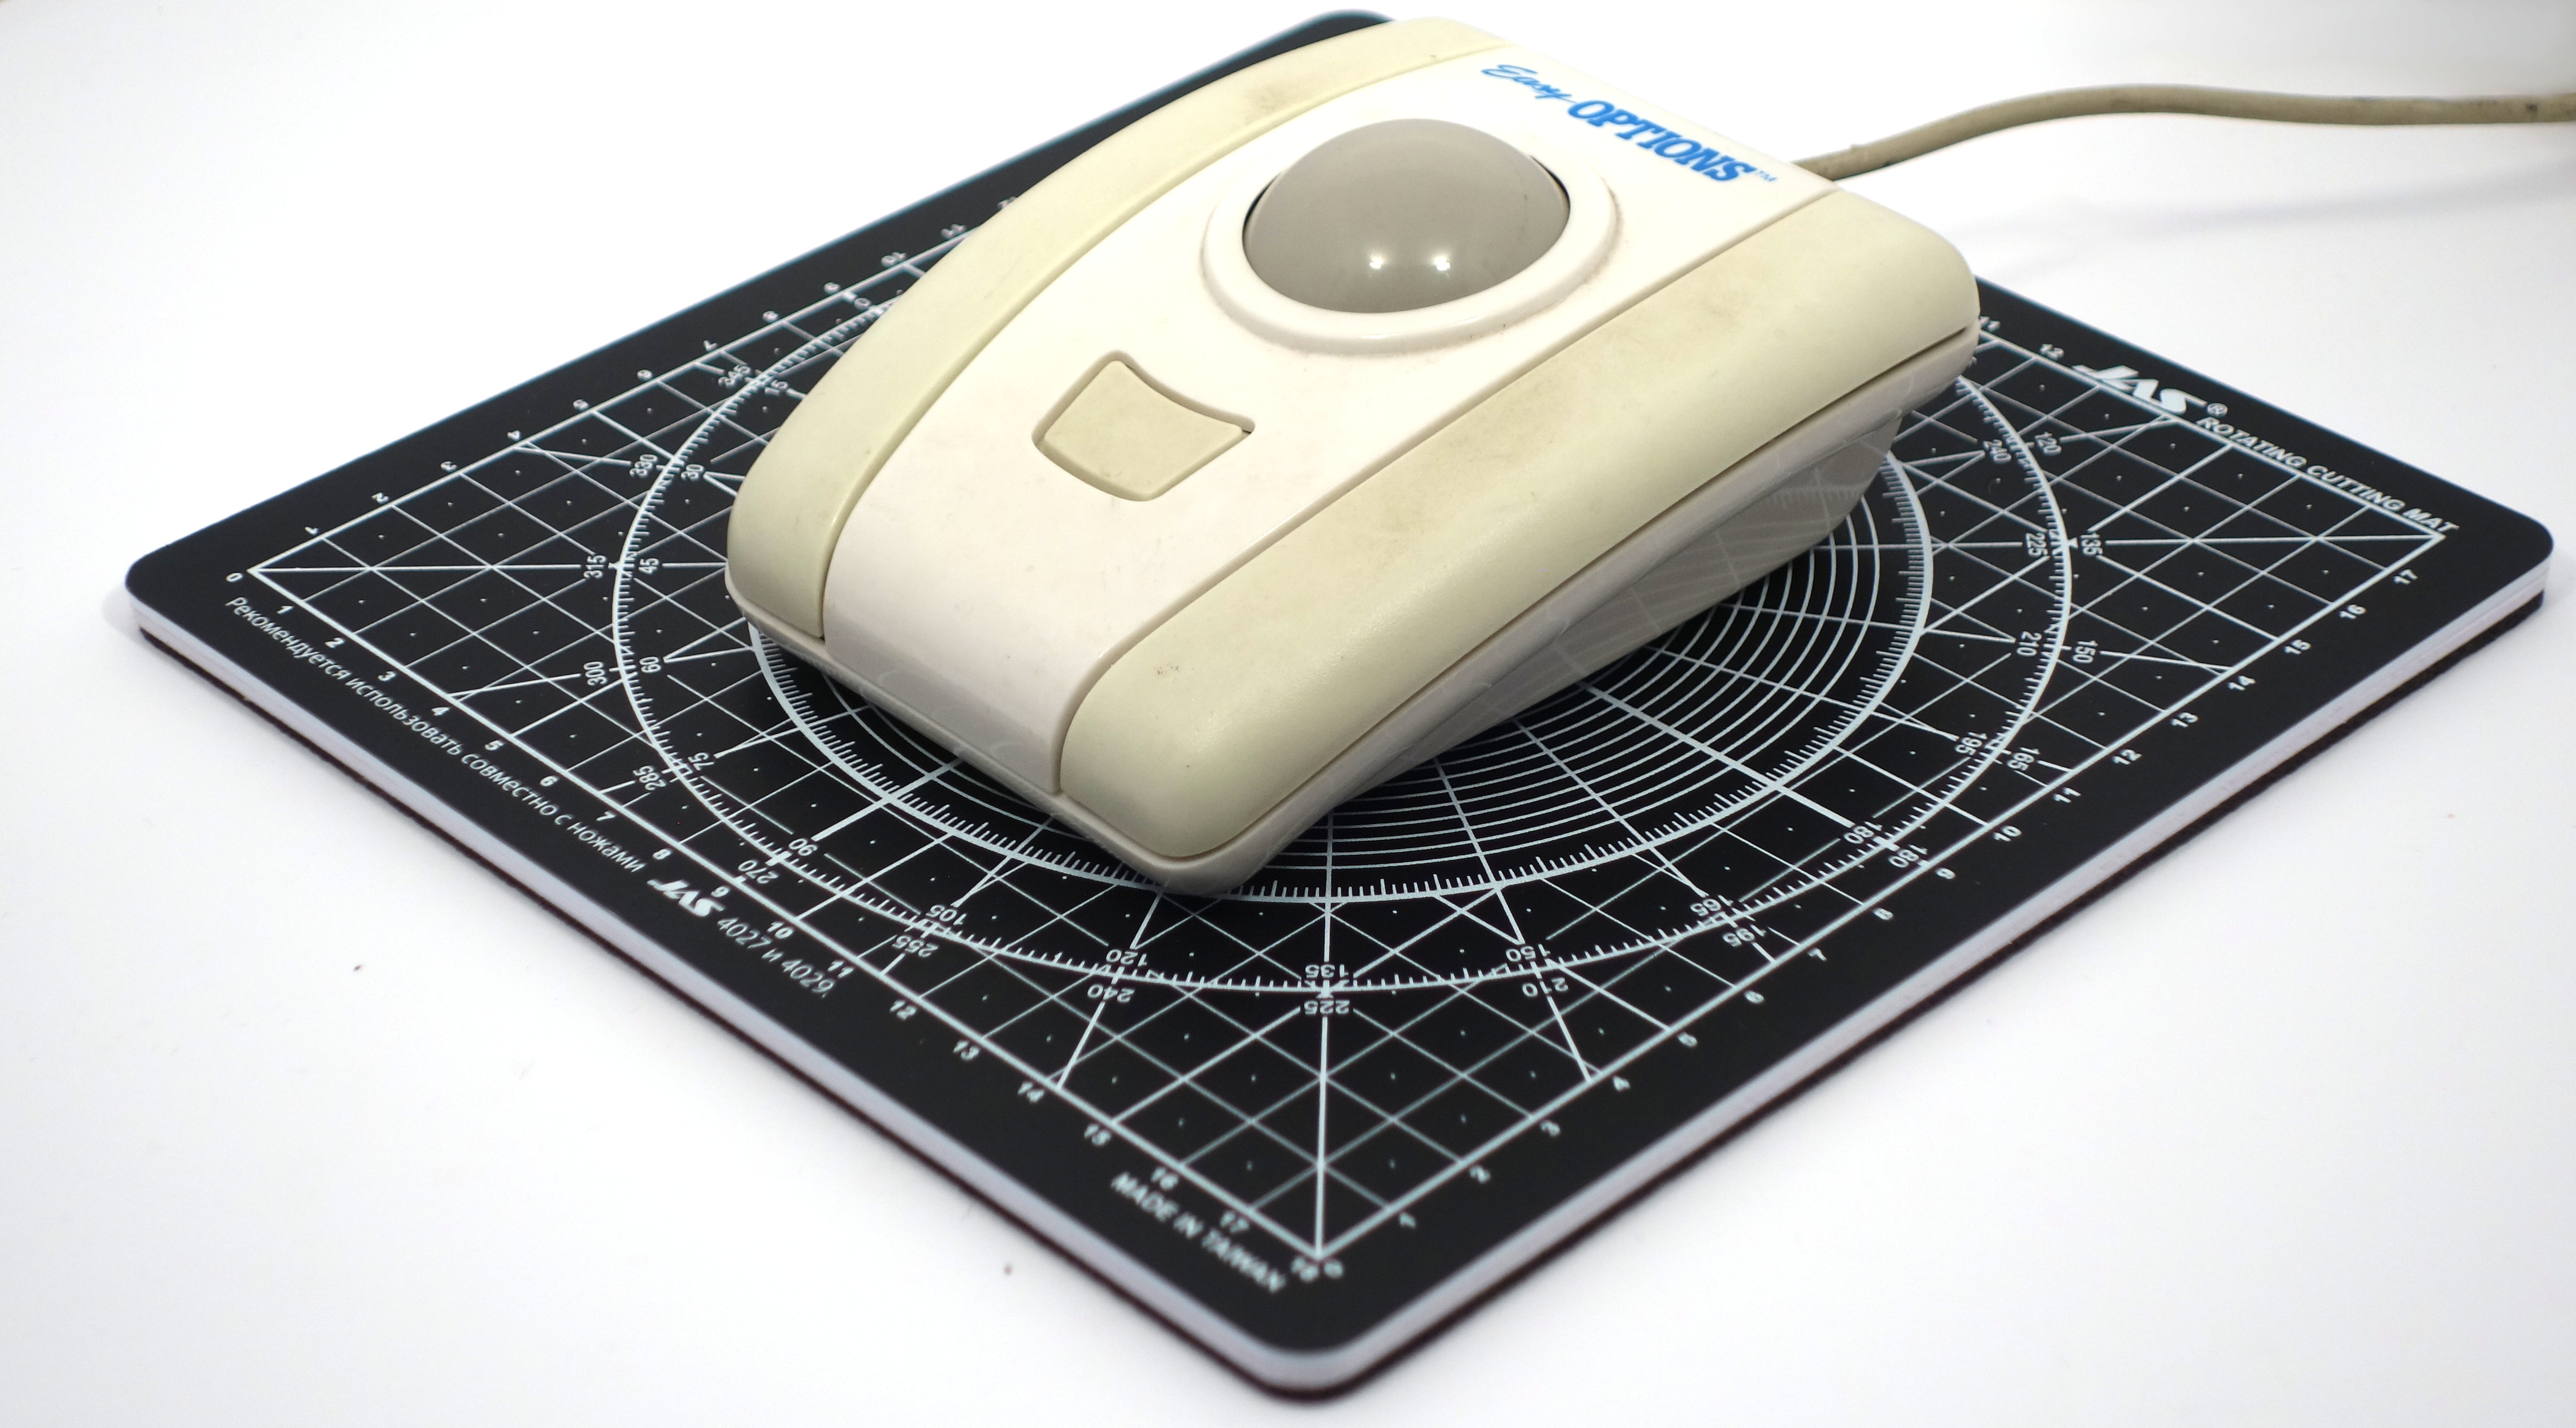
\includegraphics[scale=0.43]{1993_easy_options_trackball/size_30.jpg}
    \caption{Easy Options on a graduated pad with a grid step of 1~cm}
    \label{fig:EasyOptionsSize}
\end{figure}

In terms of ergonomics, one can note the rounded shape of the case, which practically does not have sharp corners, as well as the fact that the left and right buttons occupy its entire length, which is quite consistent with the anatomical structure of the hand (figure \ref{fig:EasyOptionsHand}).

\begin{figure}[h]
    \centering
    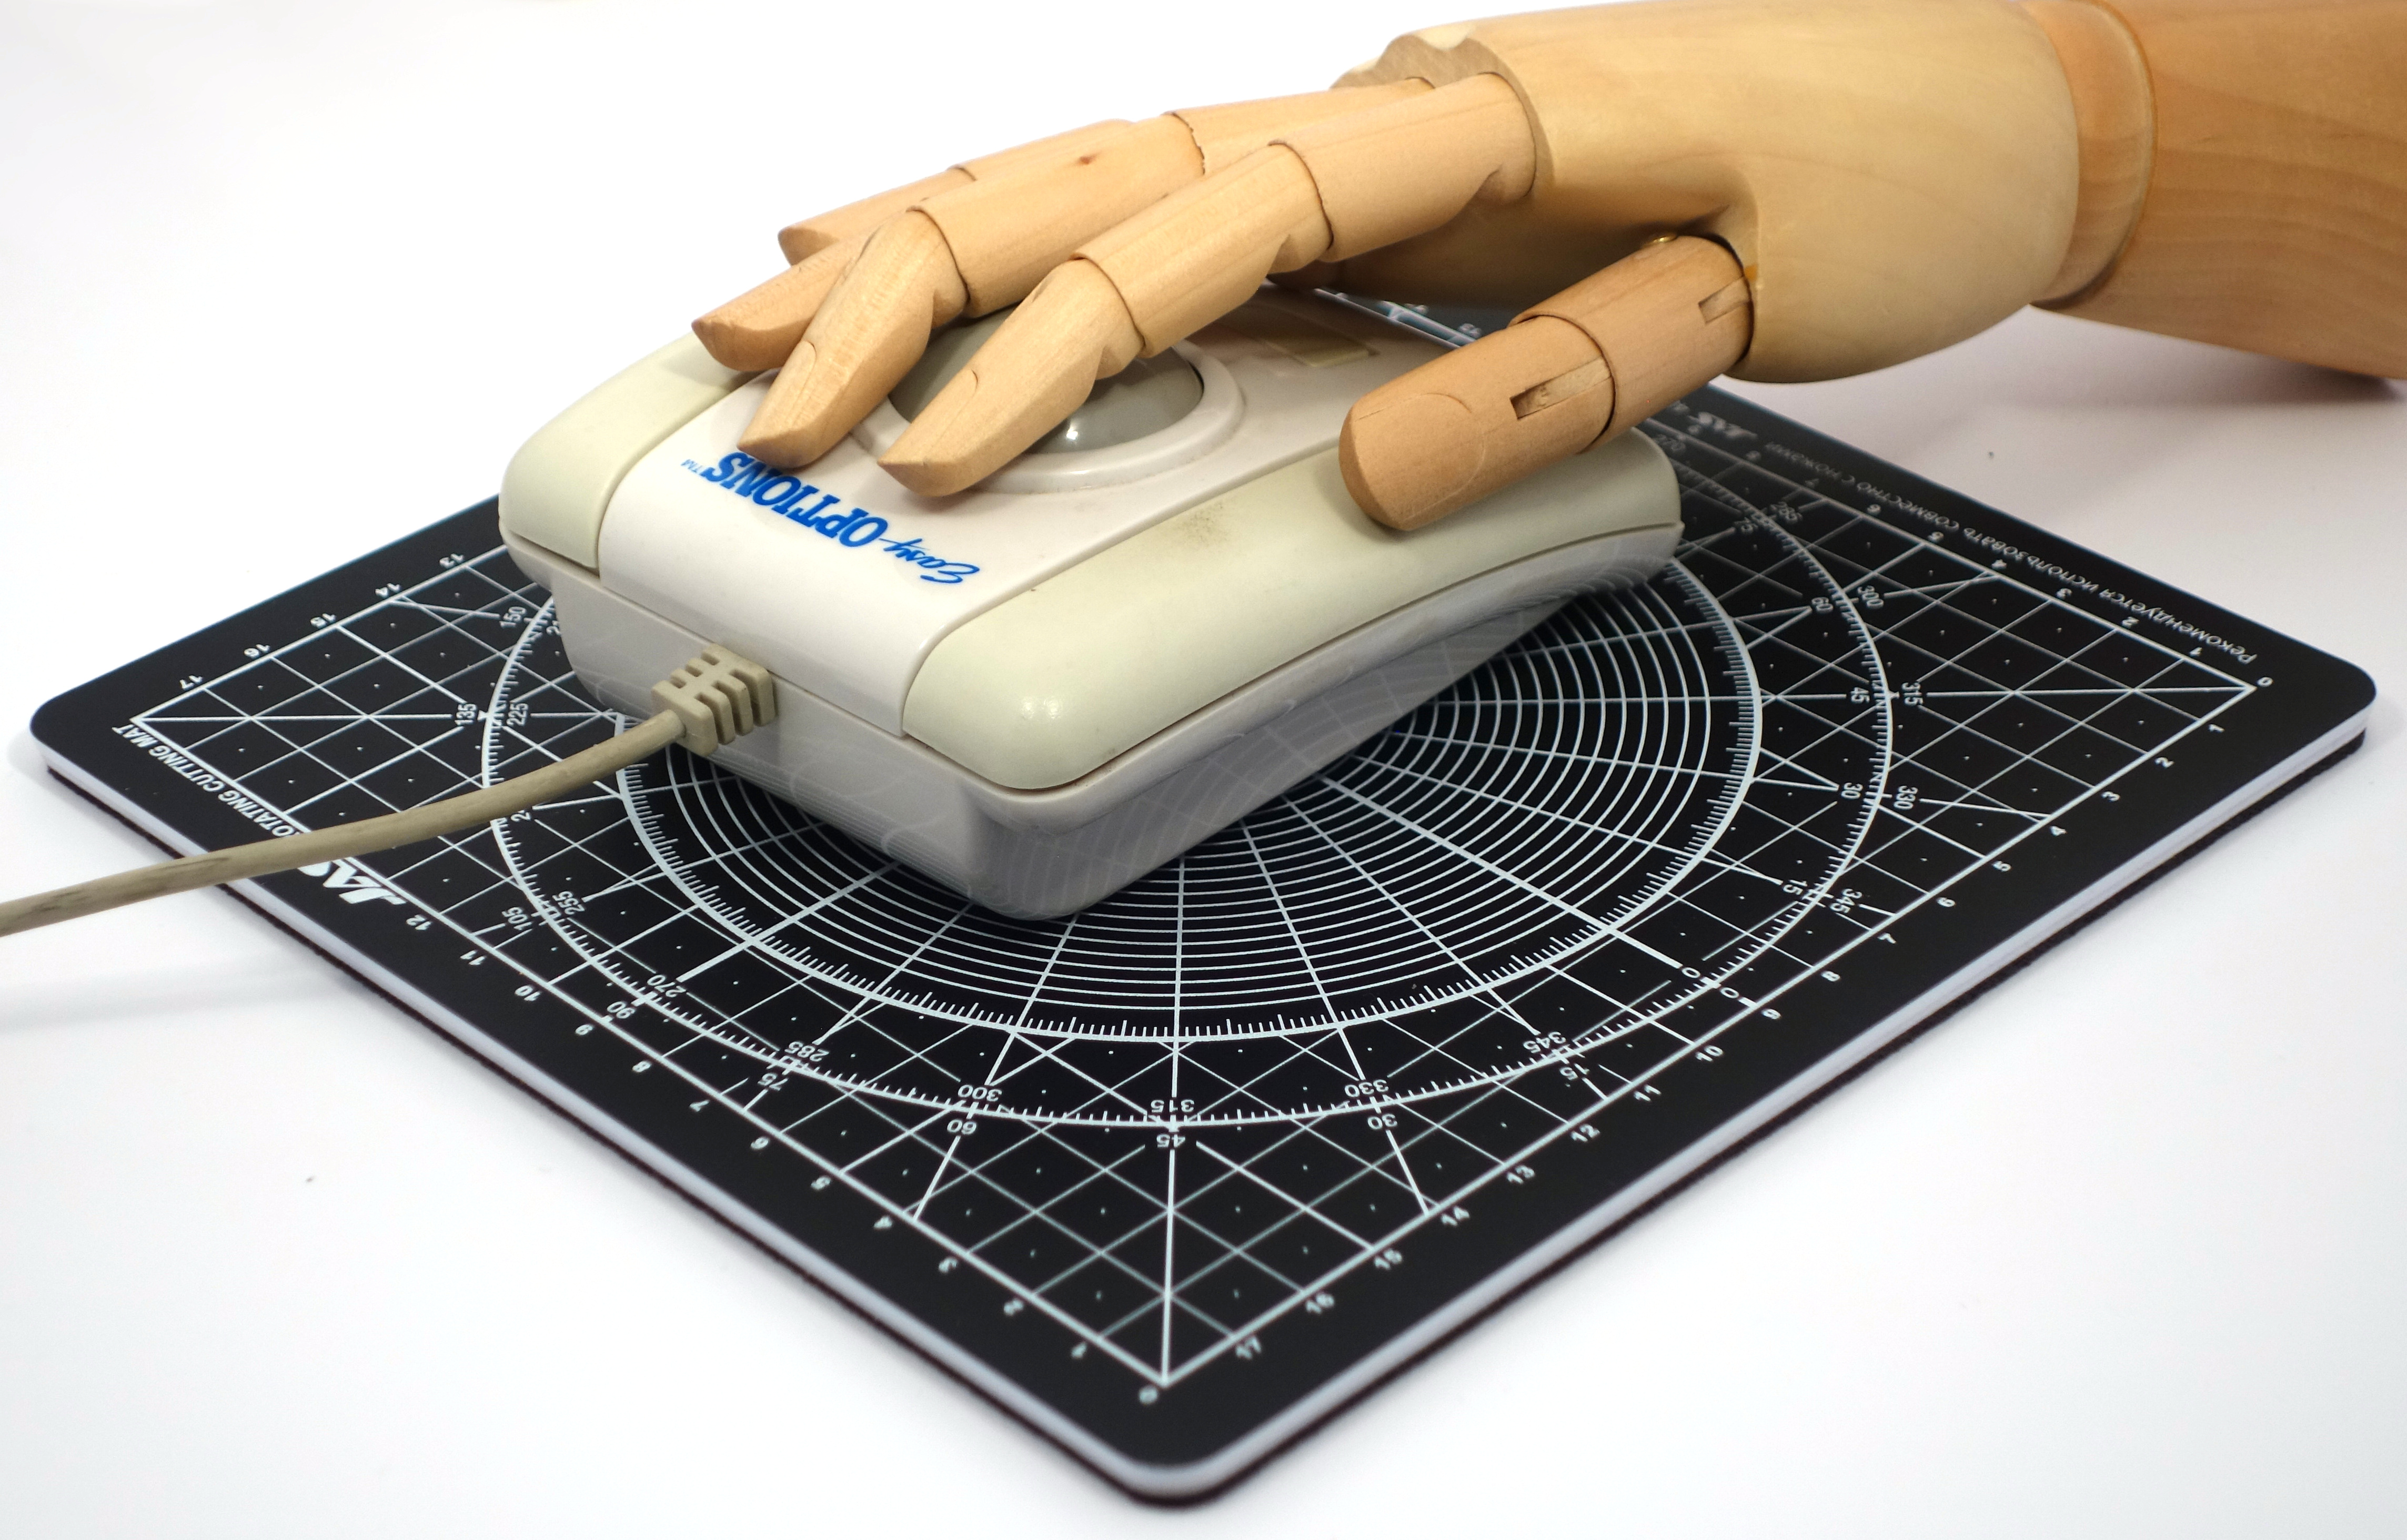
\includegraphics[scale=0.43]{1993_easy_options_trackball/hand_30.jpg}
    \caption{Easy Options with a human hand model}
    \label{fig:EasyOptionsHand}
\end{figure}

Easy Options also uses a special button that allows the user to enable or disable all other buttons to avoid accidental pressing and to conveniently move the mouse cursor, respectively. Another distinguishing feature of the manipulator is a two-way connector that can be connected to a serial port equipped with a socket with both 9 and 25 pins.

\begin{figure}[h]
    \centering
    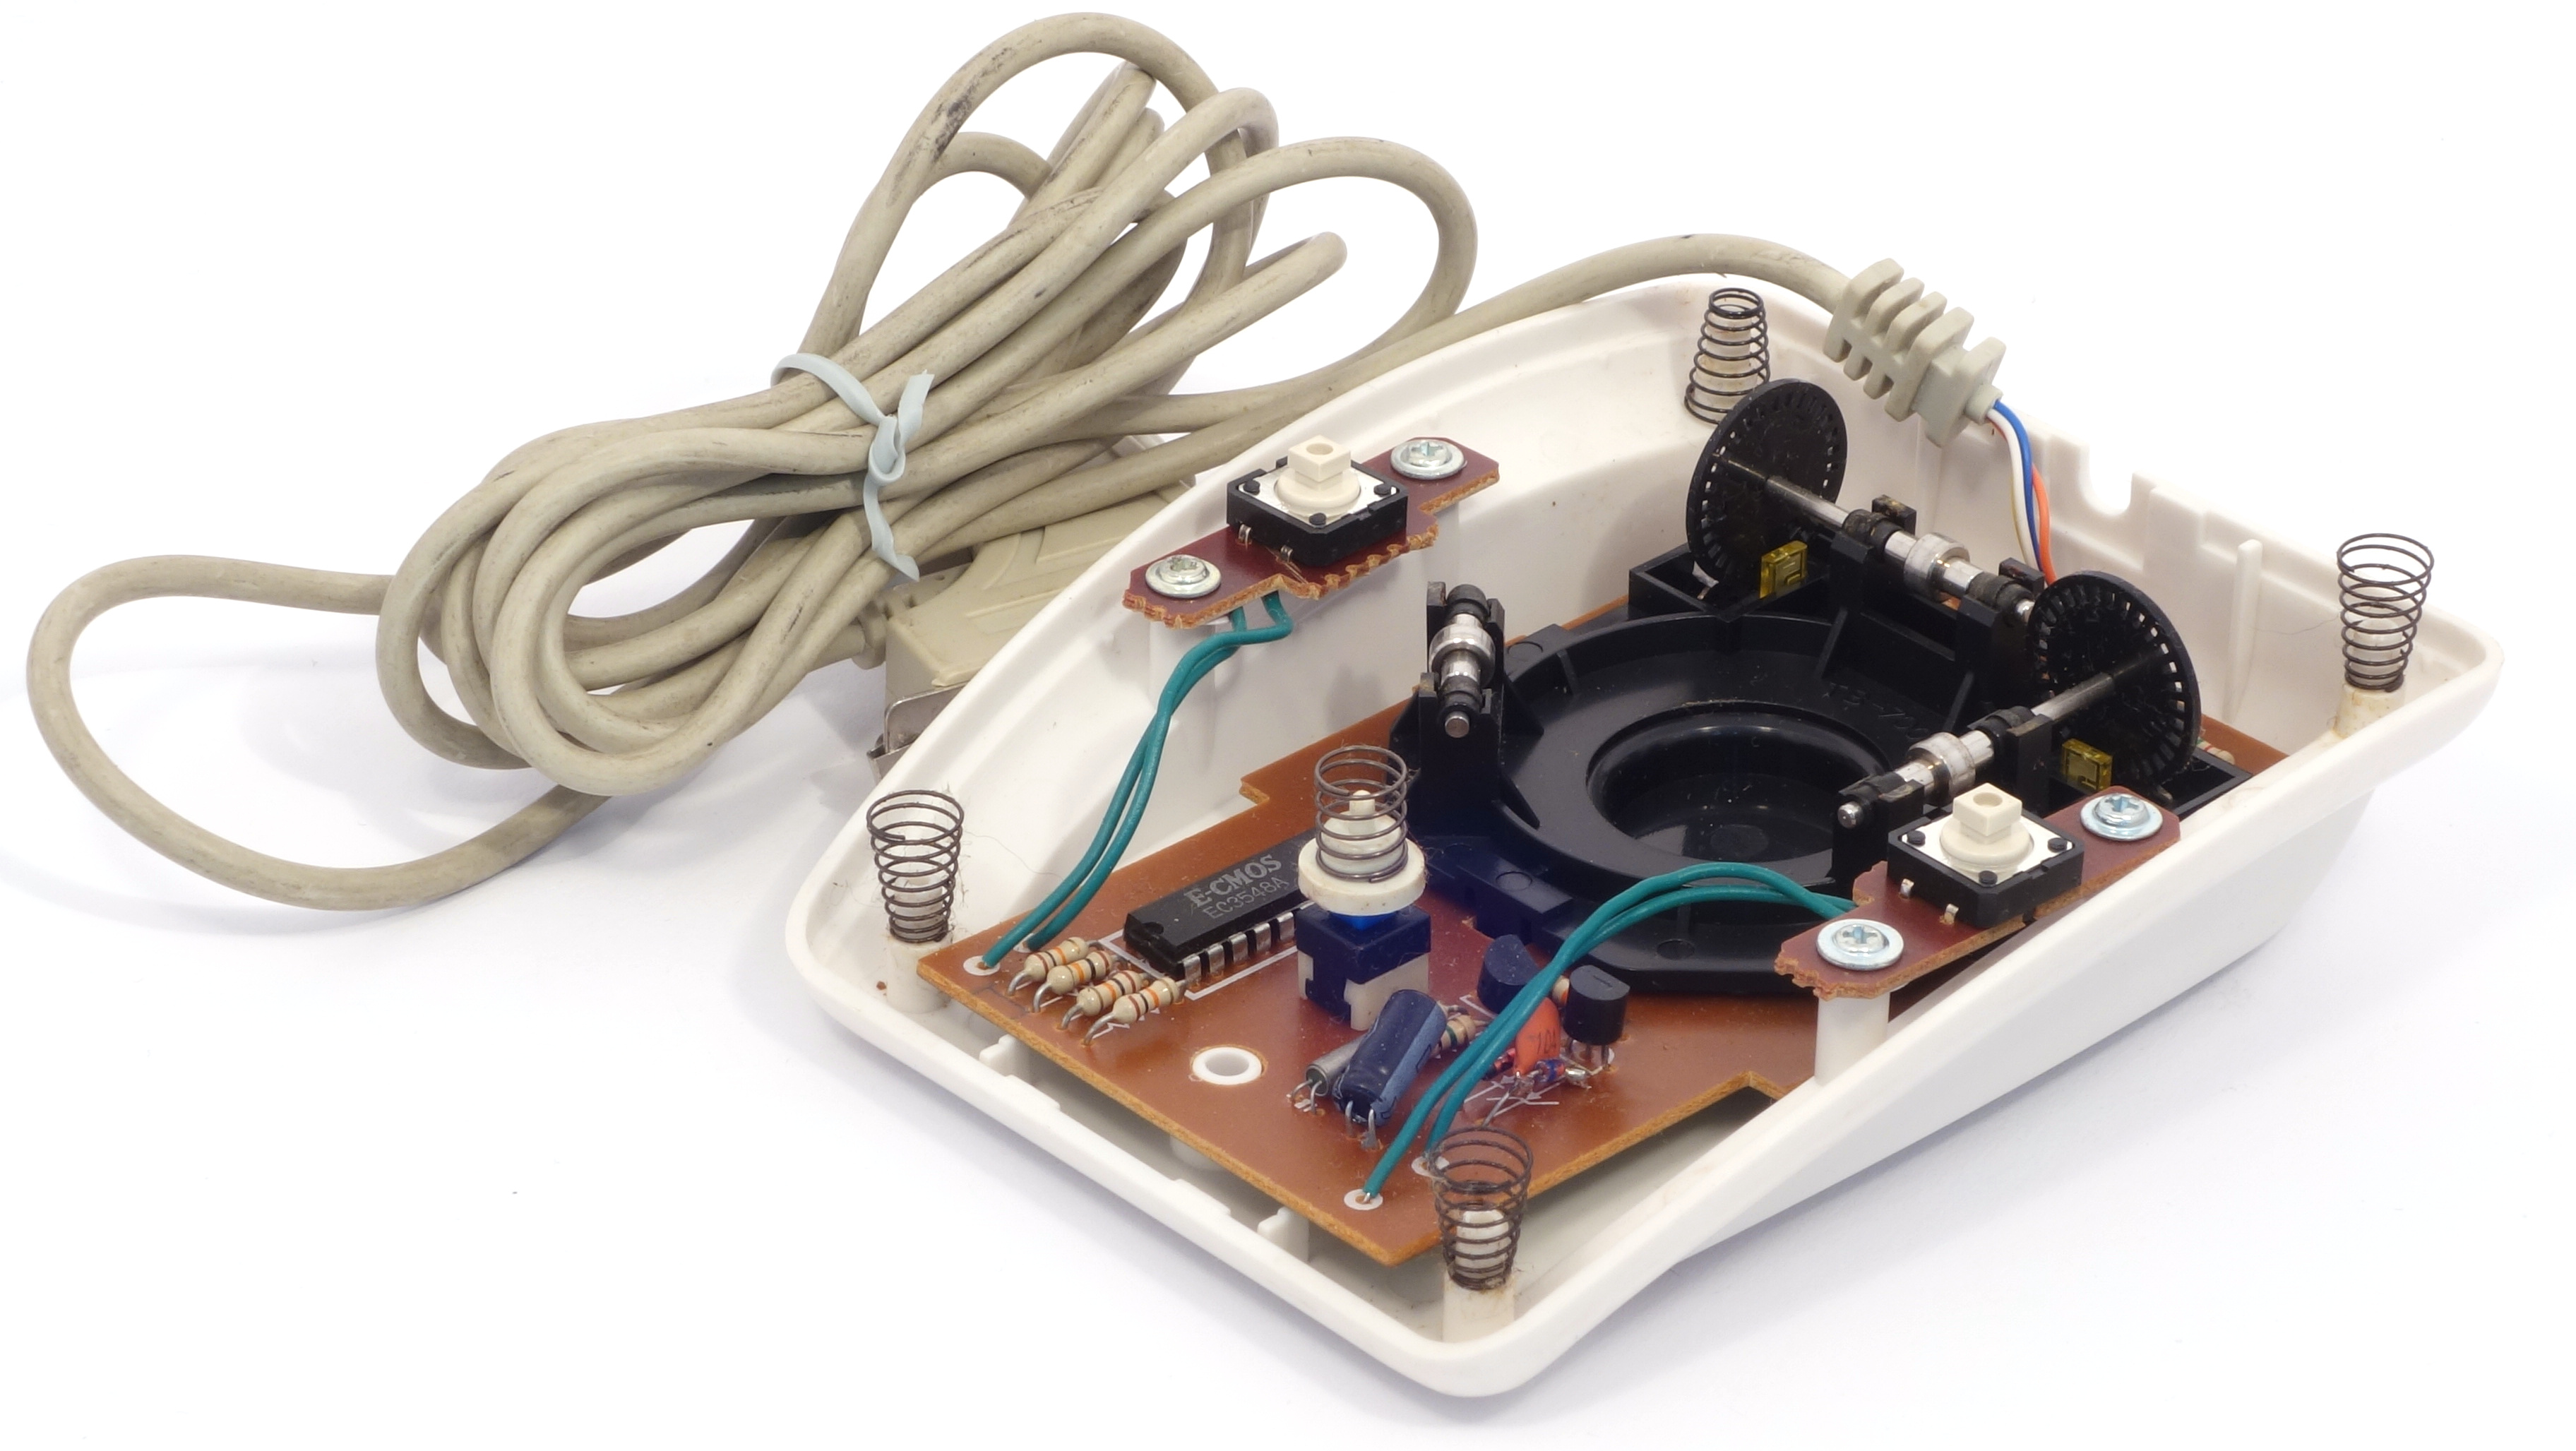
\includegraphics[scale=0.6]{1993_easy_options_trackball/inside_60.jpg}
    \caption{Easy Options disassembled}
    \label{fig:EasyOptionsInside}
\end{figure}

~

Trackball internals are shown on figure \ref{fig:EasyOptionsInside}.

As you can see, this trackball follows the traditional opto-mechanical scheme. Four springs are worthy of mention, which provide an uniform move for the long keys (left and right ones), as well as a spring-loaded central key.

\end{document}
